\section{Generative modeling 2}
\subsection{Dimensionality reduction}
Can serve as a preprocessing step to help improve results and increase speed.
Allows fro visual exploration of data and possible science discovery.
\subsubsection{Principle Components Analysos (PCA)}
PCA prioritizes the maximization of the data's variance in the embedding at the expense of local structure

Principle components are the Eigenvectors of the convariance Matrix.
Neglects the preservation of local detail.
\subsubsection{t-SNE}
\begin{figure}[!h]
    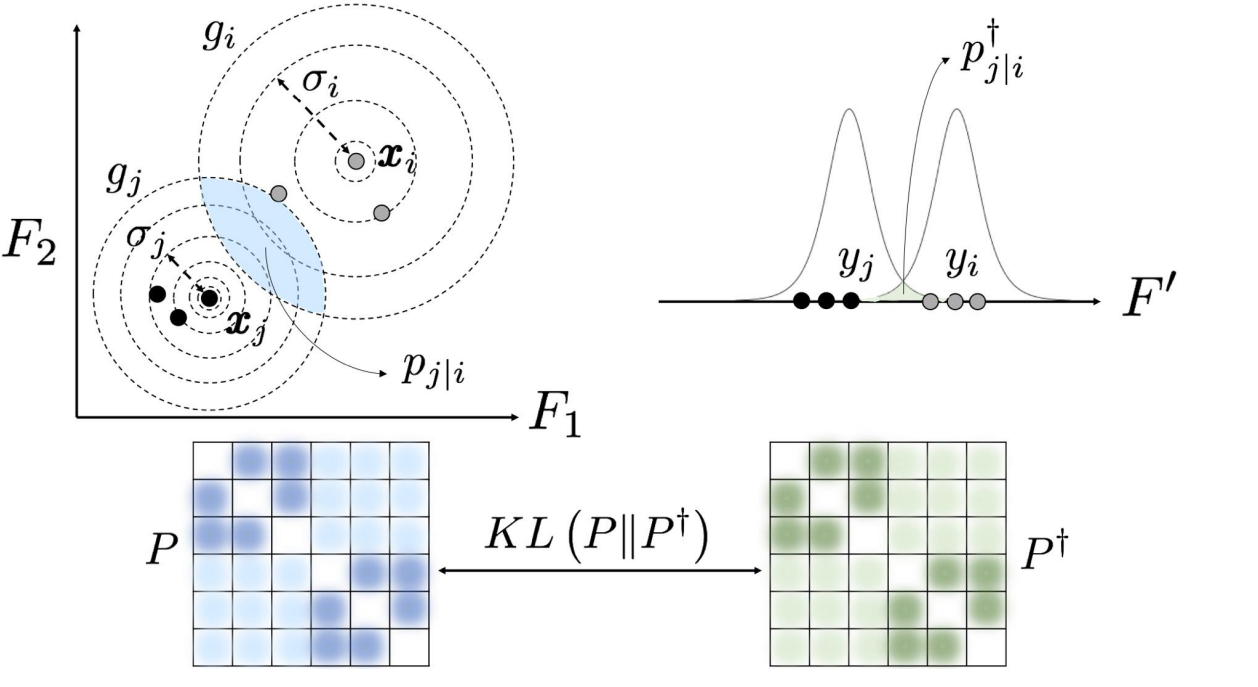
\includegraphics[width = \columnwidth]{figures/GenAI2/tSNETheory.png}
\end{figure}
\begin{itemize}
    \item Prior: Random position of n-points in 1D
    \item Loss: KL-divergence between statistical matrices.
    \item Optimization: Gradient descent + incrementally shifting 1D points
    \item Hyperparameters: perplexity
\end{itemize}

\subsubsection{Interpretation}
Playing with preplexity: Low perplexity preserves local structure, high preplexity preserves global structure, if preplexity exceeds the number of points in the dataset we get strange behaviour that should not be trusted.

Playing with convergence time and fixed perplexity: must wait until updates are relatively small. First four panels have not properly converged. If you see strange pinched shapes be cautions. Generally takes 5000 iterations.


Interpretation caution:
\begin{itemize}
    \item  Cluster sizes might not mean anything.
    \item Distance between clusters might not mean anything
    \item Random noise doesn't always look random
    \item You can see some shapes sometimes
    \item To derive topological insights you have to test many perplexities
\end{itemize}

\subsection{Variational Autoencoder (VAE)}
VAE is 
\begin{itemize}
    \item Quick for sampling
    \item Easy to train
    \item Produces blurry images
\end{itemize}

\subsubsection{Autoencoder}
\begin{itemize}
    \item Neural network trained to reproduce its input x
    \item No labels needed, unsupervised training
    \item Discover patterns in the input space and encoding them in latent space
\end{itemize}
\begin{figure}[!h]
     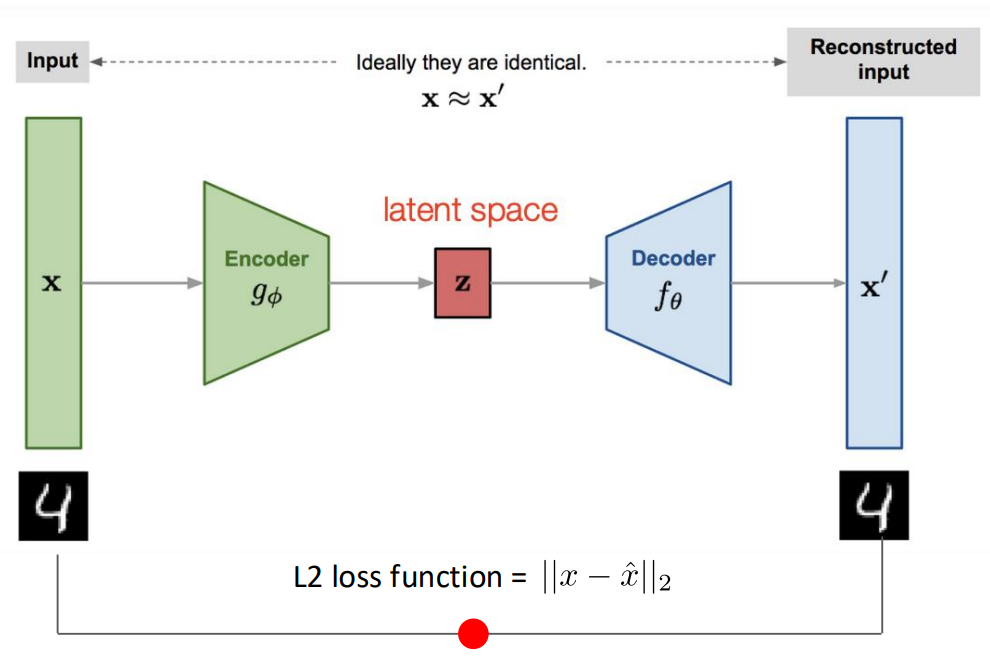
\includegraphics[width = \columnwidth]{figures/GenAI2/Autoencoder.png}
\end{figure}

Need to restrict model to learn interesting representations.
Therefore \(\text{dim}(z) < \text{dim}(x)\).

If \(\text{dim}(z) = \text{dim}(x)\) then the network would simply learn th identity matrix
 
\subsubsection*{Applications and variants}
\begin{itemize}
    \item Data Compression / Dimensionality Reduction
    \subitem Must capture most important information and compress less important information
    \item Image in-painting
    \subitem Masking during Training
    \subitem Tasked with Reconstruction
    \subitem Reconstruction Loss between predicted imgae and unmasked image
    \item De-noising, learned features robust to noise
    \item Feature extractor for downstream tasks 
\end{itemize}

Autoencoder are not generative models.
Irregular latent space prevents us from using an Autoencoder for new contect generation.

\subsection{Variational Autoencoder (VAE)}
A VAE is a probabilistic spin of an Autoencoder.

When we sample from the latent space we expect decoder to generate plausible output Reconstructions.

\subsubsection{Theory}
VAEs require three main ideas:
\begin{enumerate}
    \item Use of the evidence lower bound (ELBO) to approximate the likelihood function, leading ro a close relationship to the EM algorithm
    \item Amortized inference in which a second model, the encoder network, is used to approximate the posterior distribution over latent variable in the E step, rather than evaluating the posterior distribution for each data point exactly
    \item Making the training of the encoder model tractable using the reparameterization trick
\end{enumerate}

\subsubsection*{New objective function ELBO}
Data likelihood for continuous latent variable models
\[
p(x,\theta) = \int_{z} p_\theta(x|z)p(z)dz
\]
NN family \(f_\theta\) much more flexible function.
Intractable to compute the posterior over \(z\).
Worse than GMM because continuous.

Instead fo solving likelihood directly, we introduce a vatiational distribution to the model, the true posterior.
This allows us to split the optimization for the EM algorithm
\[
\text{log} p(x,\theta)  = \underbrace{\int_z q(z)\text{log}\left[\frac{p(x|z,\theta)p(z)}{q(z)}\right]}_{\mathcal{L}(\theta)}
\]

We want to encourage the latent space to be smooth and regular, so set the prior to a zero mean, unit-variance Gaussian.
This also allows us to derive some closed form.
\[
p(\mathbf{z}) = \mathcal{N}(\mathbf{z}|\mathbf{0,I})
\]
We drop the KL-divergence term because we have no tractable way to calculate the true posterior distribution.

The evidence lower bound (ELBO) becomes the VAE objective function that we maximize.

Contribution to the ELBO from a single data point:
\[
\mathcal{L}_n = \int q_n(\mathbf{z}_n)\text{ln}\left\{\frac{p(\mathbf{x}_n|\mathbf{z}_n,\theta)p(\mathbf{z}_n)}{q_n(\mathbf{z}_n)}\right\}d\mathbf{z}_n
\]

\( x_n \rightarrow q_n(z_n)\) data point to multi-dimensional latent distribution.
Too expensive to model \(n\) parameters distribution.
Instead of trying to evaluate a separate posterior distribution for each point train a single network called an encoer to approximate the entire posterior

\[
\mathcal{L}_n(\theta,\phi) = \int q(\mathbf{z}_n|\mathbf{x}_n,\phi) \text{ln} \left\{\frac{p(\mathbf{x}_n|\mathbf{z}_n,\theta)p(\mathbf{z}_n)}{q_n(\mathbf{z}_n|\mathbf{x}_n,\phi)}\right\}d\mathbf{z}_n
\]

\begin{figure}
    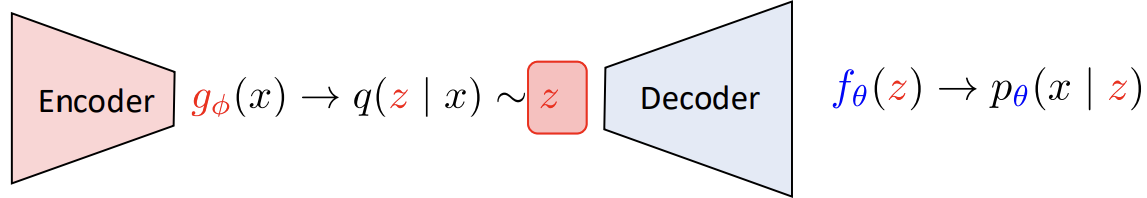
\includegraphics[width = \columnwidth]{figures/GenAI2/ELBO.png}
\end{figure}

VAE only maximizes the ELBO.
Since we only approximate the true posterior distribution with an encoder, we will always be equal or less than the likelihood.
Analogy.

E-Step: Fixed decoder, improve posterior approximation with encoder.

M-Step: Fixed encoder, increase value of the ELBO by optimizing the decoder.

Rewrite ELBO using log function and Bayes law and definition of KL-divergence:

\[
\mathcal{L}_n(\theta,\phi) = \int q(\mathbf{z}_n|\mathbf{x}_n,\phi)  \text{ln}  p(\mathbf{x}_n|\mathbf{z}_n,\theta) d\mathbf{z}_n - \text{KL}(q_n(\mathbf{z}_n|\mathbf{x}_n,\phi)||p(\mathbf{z}_n))
\]

If our encoder network models a Gaussian distribution then the KL term has a simple an analytic expression.
\[
q(\mathbf{z}|\mathbf{x},\mathbf{\phi}) = \prod_{j = 1}^{M}\mathcal{N}(z_j|\mu_j(\mathbf{x},\mathbf{\phi}),\sigma_j^2(\mathbf{x},\mathbf{\phi}))
\]

\[
\text{KL}(q_n(\mathbf{z}_n|\mathbf{x}_n,\phi)||p(\mathbf{z}_n)) = \frac{1}{2}\sum_{j=1}^{M}\left\{1+ln\sigma_j^2(\mathbf{x}_n) - \mu_j^2(\mathbf{x}_n)-\sigma_j^2(\mathbf{x}_n)\right\}
\]

Still cannot directly evaluate this term over all \(z\) so use Monte Carlo estimate
\[
    \int q(\mathbf{z}_n|\mathbf{x}_n,\phi)  \text{ln}  p(\mathbf{x}_n|\mathbf{z}_n,\theta) d\mathbf{z}_n \approx \frac{1}{L}\sum_{l = 1}^{L} p(\mathbf{x}_n|\mathbf{z}_n^{(l)},\theta)
\]

Monte Carlo requires us to randomly sample from the encoder, but how do we take the gradient of a stochastic variable?

For decoding, we need to sample from \(p_\theta(\mathbf{x}|z)\) for latent variable \(z \sim q_\theta(z|\mathbf{x})\).
We let endcoder network predict \(\mu(x),\sigma(x)\).
Then we can sample standard normal random vectors \(\epsilon \sim \mathcal{N}_d(0,1)\) and set \(z = \mu + \sigma \odot \epsilon\).

This allows us to remove the stochasticity from the model and use gradient based optimization to learn parameters for both the encoder and decoder networks.

Finally the full loss function for the VAE becomes:
\[
\mathcal{L} = ||x-\hat{x}|| + \frac{1}{2}\sum_{i}\left\{ 1 + \text{ln} \sigma_i^2 - \mu_i^2 - \sigma_i^2\right\}
\]

Reconstructed \(\hat{x}\) depends on parameters of encoder and decoder networks \(\phi\) and \(\theta\).

Output of the encoder network, \(\mu_i(x),logvar_i(x)\) depend on the parameters of the encoder network, \(\phi\).

\subsection{Diffusion models}
Diffusion models are:
\begin{itemize}
    \item Expensive to sample
    \item Easy to train
    \item Produces high quality images
\end{itemize}

The idea of Diffusion model is based on two key steps
\begin{itemize}
    \item Forward(noising) process 
    \item Backward(denoising) process
\end{itemize}
Goal: Predict the added noise and then remove it.

The loss is the difference between the predicted noise and the added noise:
\[
L_t = ||\epsilon_t-\epsilon_\theta(x_t,t)||^2
\]

\begin{figure}[!h]
    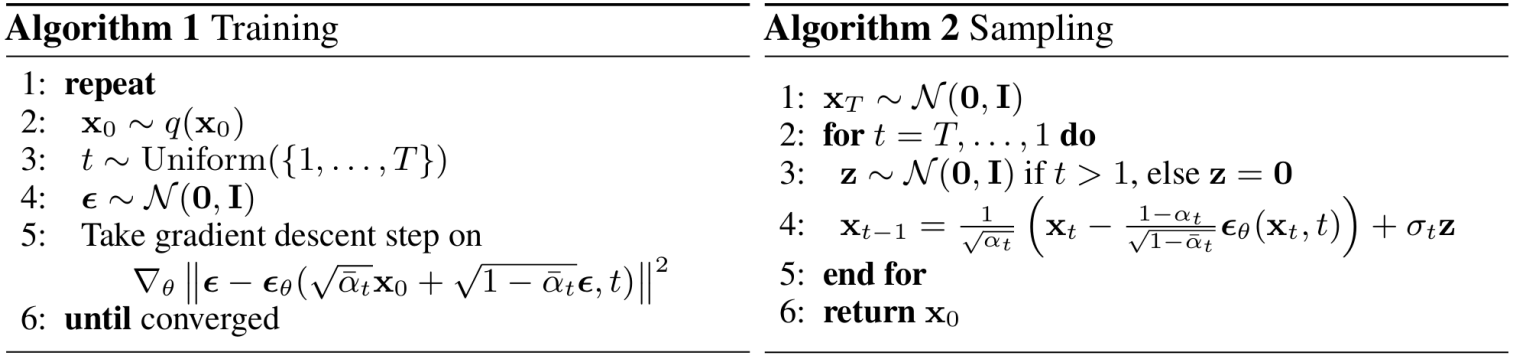
\includegraphics[width = \columnwidth]{figures/GenAI2/DiffusionAlgorithm.png}
\end{figure}